\chapter{State of the Art}
\label{ch:State of the Art}

As described in \autoref{ch:Introduction}, the main contribution of this work is to provide a novel approach allowing to modify specific \acrshort*{RDF} values by moving cards over a Kanban board. Since there is no comparable previous work, this chapter provides an overview of the visualization of \acrshort*{RDF} graphs (\autoref{sec:Graph Visualization}), as well as existing Kanban board solutions (\autoref{sec:Kanban Board Solutions}).

\section{Graph Visualization}\label{sec:Graph Visualization}

As mentioned in the introduction, graphs are usually visualized by a set of ellipses that are interconnected by arrows, representing the graphs’ nodes and edges, respectively. Nodes, however, may also be shaped as rectangles depending on their context. A notable application for editing and visualizing RDF resources is \textit{Protégé}.\footnote{Initial Release: 1999. GitHub: \url{https://github.com/protegeproject/protege}. Web-version: \url{https://webprotege.stanford.edu/}.} Since its initial release in 1999, it has become the leading ontological engineering tool. It is an open-source project, and its plugin system allows other developers to contribute to the project \parencite[62]{Gasevic2009}.

Another more recent work in the field of visualizing linked data (especially ontologies) has been conducted by Lohmann and colleagues (\citeyear{Lohmann2016}). The authors introduced a visual language for \acrshort*{OWL} ontologies (\textit{\tracknshrink{VO\kern-0.2ptWL}}) aiming to provide a comprehensive visualization that is comprehensible by \textit{“[\textellipsis] casual ontology users with only little training”} \parencite[1]{Lohmann2016}. \tracknshrink{VO\kern-0.2ptWL} is implemented as a Protégé plugin as well as a web application.\footnote{\tracknshrink{\textit{VO\kern-0.2ptWL}} home page: \url{http://vowl.visualdataweb.org/}.} The web application is publicly available as an open-source project\footnote{More information: \url{http://vowl.visualdataweb.org/webvowl.html}} and can be embedded by other applications. For example, \tracknshrink{VOWL} is integrated within eccenca’s front-end (i.e., the \textit{DataManager}).

Furthermore, \citeauthor{Lohmann2016} elaborated on existing graph visualization in their work, most of which are available as Protégé plugins; for example, \textit{TGViz},\footnote{Protégé Wiki: \url{https://protegewiki.stanford.edu/wiki/TGViz}.} \textit{Navig\tracknshrink{O\kern-0.2ptWL}},\footnote{Protégé Wiki: \url{https://protegewiki.stanford.edu/wiki/NavigOWL}.} and \textit{\tracknshrink{SO\kern-0.3ptVA}}.\footnote{Protégé Wiki: \url{https://protegewiki.stanford.edu/wiki/SOVA}.} A comprehensive review of knowledge graph visualizations is provided in section two in the article (\cite[2]{Lohmann2016}). 

It should be again pointed out, that this work does not attempt to visualize an entire graph. This approach would primarily lead to a clash of paradigms. It would map a graph to a relational model since a Kanban board can be considered as a table structure. However, when a user defines the structural components of the board (i.e., the resources which should be used for cards, columns, and lanes within the board configuration, see \tracknshrink{FR}\textsubscript{1}), they explicitly dissect the graph, and therefore, bypassing the clash. In other words, preselecting the board components creates a table-compatible subset graph.

\newpage

\noindent To illustrate the mapping and visualization process of the \tns{RMB}. \autoref{fig:VOWL} (A1) compares a `traditional' graph visualization (using \tracknshrink{VOWL})\footnote{The \tracknshrink{VOWL} \acrshort*{FOAF} visualization can be accessed under \url{http://www.visualdataweb.de/webvowl/\#foaf}.} with a mockup of the \acrlong*{RMB} (B). Both images (A1) and (B), depict a small section of the \acrshort*{FOAF} graph, whereas (A2) reveals details about a selected node from (A1); in this instance, the \acrshort*{FOAF} term \textit{knows} got selected. On the other hand, (B) depicts a small section from the first use case of this work (i.e., \acrshort*{FOAF} Term Status). As stated before, the \acrshort*{RMB} only targets selected card classes and maps their inherent properties to the columns and lanes of the board. Thus, in contrast to other graph visualizations, the \acrshort*{RMB} provides a selective perspective on a graph. 

To comprehend the mapping and visualization process of the \acrshort*{RMB}, compare the contents of image (A2) and (B) of \autoref{fig:VOWL}. In the first use case, the prototype’s aim was to target three specific properties of the \acrshort*{FOAF} graph in order to generate a board. These three properties (i.e., cards, columns, and lanes) were defined as \textit{board component resources}, as they structurally define the board components. The card classes were defined as one of \acrshort{owl}\texttt{Class}, \acrshort{owl}\texttt{ObjectProperty}, or \acrshort{owl}\texttt{DatatypeProperty}. Therefore, the term \textit{knows} appeared as a card on the board, as in image (B) and listed in (A2). The type property was also used to separate the cards by lane. Finally, the cards got distributed over columns by their inherent \acrshort{vs}\texttt{term\_status} value, as depicted in (B) and listed in (A2).

\begin{figure}[ht]
	\centering \begin{tikzpicture}
	\node[anchor=south west,inner sep=0] (image) at (0,0,0) {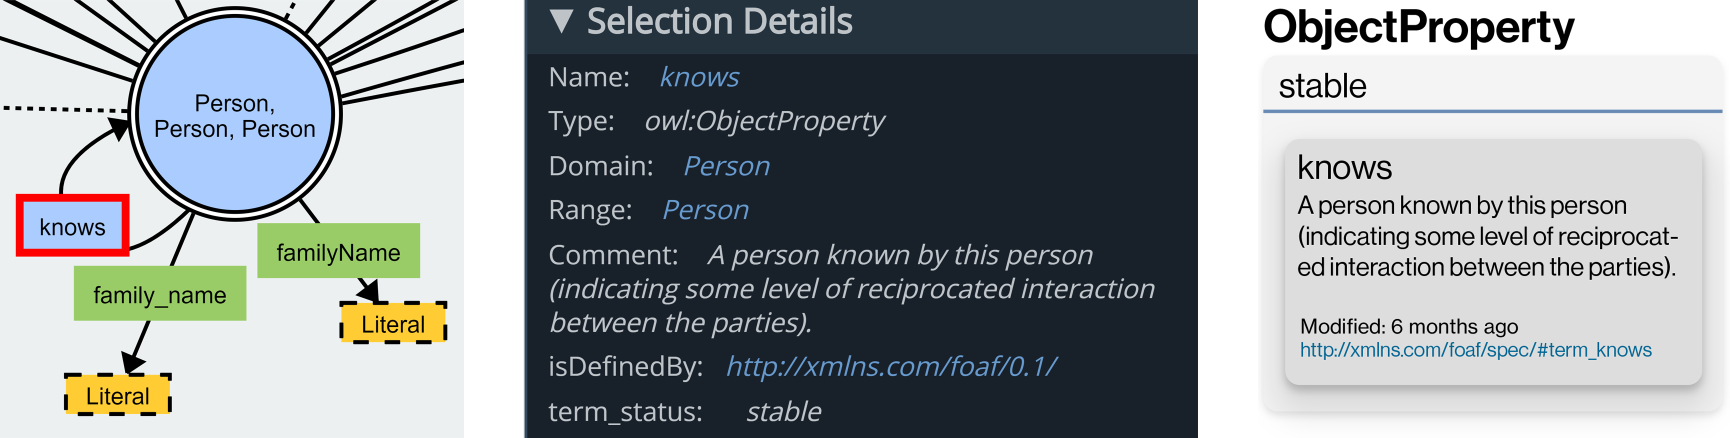
\includegraphics{img/vowl.png}};
	\begin{scope}[x={(image.south east)},y={(image.north west)}]
% 	% next four lines will help you to locate the point needed by forming a grid. comment these four lines in the final picture.↓
% 		\draw[help lines,xstep=.1,ystep=.1] (0,0) grid (1,1);
% 		\draw[help lines,xstep=.05,ystep=.05] (0,0) grid (1,1);
% 		\foreach \x in {0,1,...,9} { \node [anchor=north] at (\x/10,0) {0.\x}; }
% 		\foreach \y in {0,1,...,9} { \node [anchor=east] at (0,\y/10) {0.\y};}
% 	% upto here↑
	



	\draw (0.110,1.100) node[anchor=west] {(A1)};
	\draw (0.468,1.100) node[anchor=west] {(A2)};
	\draw (0.842,1.100) node[anchor=west] {(B)};
	
	\end{scope}
	\end{tikzpicture}
	\caption[Visualization Approaches of \tracknshrink{VOWL} and the \acrshort*{RMB}]{Visualization approaches of \tracknshrink{VOWL} (A) and the \acrshort*{RMB} (B). \tracknshrink{VOWL} provides a visualization for the entire graph, whereas the \acrshort*{RMB} targets a specific selection.}
	\label{fig:VOWL}
\end{figure}





\section{Kanban Board Solutions}\label{sec:Kanban Board Solutions}


The initial idea of this project was to develop an in-house Kanban board from scratch. However, considering that the Kanban board acts only as a tool for reaching the actual project goal, we decided to use the existing Kanban board solution react-trello as underlying basis. This decision was mainly based on the assumption that developing a board from scratch would go beyond the scope of a Master’s thesis. Compared to an in-house application, a third-party solution would allow to develop a vertical prototype at a faster pace while focusing on the actual goal of the project. Furthermore, an in-house board solution would bear the risk of stagnation once the basic requirements were satisfied. 

To explain why we chose react trello as basis, the current section reviews existing implementations of Kanban board solutions. Our review was based on the following project-relevant criteria: First and foremost, a permissive software license (such as \tracknshrink{MIT} or \tracknshrink{ISC}) is essential for a component that is supposed to be integrated into a commercial software product. Moreover---having the technology stack in mind---the eccenca’s user interface is created with React, meaning that the Kanban board needed to be React-based. React can be used with both languages JavaScript and TypeScript. Although both languages allow to develop an independent software component, JavaScript represents the preferred option, since eccenca’s build workflows and front-end codebase is entirely written in and adjusted towards JavaScript. Another crucial criterion was the injectability of data. As mentioned previously, our project did not aim to create data from scratch. Instead, existing data needs to be integrated into the board.

We only considered active projects, that is projects with the last commit date no longer than one year ago. As an indicator of popularity and quality, we used the star and fork count. \autoref{tab:Kanban Board Comparison} provides an overview of publicly available Kanban board solutions. Projects set in bold type are fulfilling most of the just criteria.

\begin{table}[H]
\small
\libertineLF
\centering
\begin{tabular}{lllll}
\toprule
\begin{tabular}[t]{@{}l@{}}Project, \textit{License}, Author\\{\footnotesize GitHub Page}\end{tabular}                                                     & \begin{tabular}[t]{@{}l@{}}JS/TS\\{\footnotesize React Version}\end{tabular}             & \begin{tabular}[t]{@{}l@{}}Injectable?\\{\footnotesize Source}\end{tabular} & Lanes? & Stars/Forks \\
\midrule
\begin{tabular}[t]{@{}l@{}}\textbf{react-kanban, \textit{\tracknshrink{MIT}}, Lourenci, Leandro}\\ {\scriptsize \url{ https://github.com/lourenci/react-kanban}}\end{tabular}           & \begin{tabular}[t]{@{}l@{}}\textbf{JavaScript}\\ {\footnotesize \textbf{\textgreater{}16.8.5}}\end{tabular} & \begin{tabular}[t]{@{}l@{}}\textbf{Yes}\\{\footnotesize \textbf{JSON-like}}\end{tabular}      & \textbf{No}    & \textbf{61/19}  \\ \addlinespace
\begin{tabular}[t]{@{}l@{}}React Kanban \tracknshrink{DND}, \textit{\tracknshrink{MIT}}, Besen, Lucas\\ {\scriptsize \url{ https://github.com/lucasbesen/react-kanban-dnd}}\end{tabular} & \begin{tabular}[t]{@{}l@{}}TypeScript\\ {\footnotesize \textgreater{}16.5.2}\end{tabular} & \begin{tabular}[t]{@{}l@{}}Yes\\{\footnotesize \acrshort*{JSON}-like}\end{tabular}      & No     & 95/10       \\ \addlinespace
\begin{tabular}[t]{@{}l@{}}\textbf{react-trello, \textit{\tracknshrink{MIT}}, Ramachandran, R.}\\ {\scriptsize \url{ https://github.com/rcdexta/react-trello}}\end{tabular}            & \begin{tabular}[t]{@{}l@{}}\textbf{JavaScript}\\ {\footnotesize \textbf{\textgreater{}15.4.2}}\end{tabular} & \begin{tabular}[t]{@{}l@{}}\textbf{Yes}\\{\footnotesize \textbf{JSON-like}}\end{tabular}      & \textbf{No}     & \textbf{781/192}     \\ \addlinespace
\begin{tabular}[t]{@{}l@{}}Kanban Board App, \textit{\tracknshrink{ISC}}, Shellyl, N.\\ {\scriptsize \url{ https://github.com/shellyln/kanban-board-app}}\end{tabular}   & \begin{tabular}[t]{@{}l@{}}TypeScript\\ {\footnotesize \textgreater{}16.9.0}\end{tabular} & \begin{tabular}[t]{@{}l@{}}No\\{\footnotesize Couch\tracknshrink{DB}}\end{tabular}         & Yes    & 16/5         \\ \addlinespace
\begin{tabular}[t]{@{}l@{}}React Kanban, \textit{\tracknshrink{MIT}}, Englund, Markus\\ {\scriptsize \url{ https://github.com/markusenglund/react-kanban}}\end{tabular}      & \begin{tabular}[t]{@{}l@{}}JavaScript\\ {\footnotesize \textgreater{}16.2.0}\end{tabular} & \begin{tabular}[t]{@{}l@{}}No\\{\footnotesize Mongo\tracknshrink{DB}}\end{tabular}         & No     & 1,400/140   \\ 
\bottomrule
\end{tabular}
\caption[Comparison of React Kanban Board Solutions]{Comparison of React Kanban board solutions based on their development language, data injectability, swimlane support, star, and fork count.}
\label{tab:Kanban Board Comparison}
\end{table}


\noindent As illustrated in \autoref{tab:Kanban Board Comparison}, react-kanban (first commit on March 19, 2019) and react-trello (first commit on January 24, 2017) turned out to be the most promising projects to provide a foundation for this work. Both React projects are under active development, and share the advantages of being JavaScript-based, and offering an interface to inject data. On the other hand, both projects, by design, do not support swimlanes. A central advantage of react-trello is, that it has higher popularity and active contributor count compared to react-kanban. Moreover, at the time of developing, eccenca’s React codebase is at version 15.x, making it an excellent bedrock, since its minimal supported version is React 15.4.2. Furthermore, react-trello seems to be a sophisticated project with active contributions from over 20 users, and active maintenance regarding its issue management on GitHub.





